\documentclass[tikz,border=10pt]{standalone}
\usepackage[scaled=0.95]{helvet}
\renewcommand{\familydefault}{\sfdefault}
\usepackage[europeanresistors,americanvoltages]{circuitikz}
\definecolor{TEJNavy}{HTML}{1E2B55}
\definecolor{TEJBlue}{HTML}{1769AA}
\definecolor{TEJGold}{HTML}{D49B19}
\begin{document}
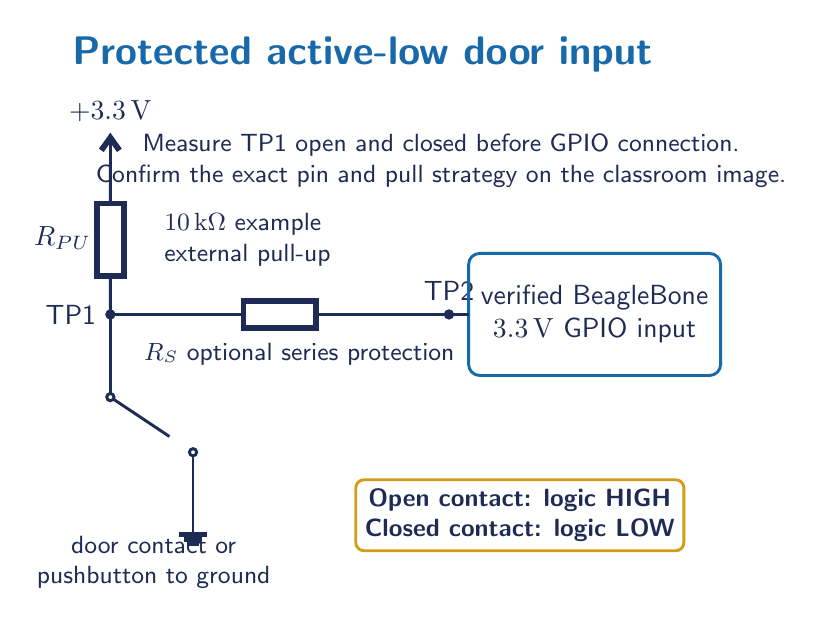
\begin{tikzpicture}[line width=1.05pt,draw=TEJNavy,text=TEJNavy,font=\sffamily]
  \ctikzset{bipoles/length=1.15cm}
  \node[font=\bfseries\Large,text=TEJBlue] at (5.3,6.6)
    {Protected active-low door input};

  \draw (2.1,5.2) node[vcc] {$+3.3\,\mathrm{V}$}
    to[R,l_={$R_{PU}$}] (2.1,3.3)
    node[circ,label=left:{TP1}] (input) {};
  \node[anchor=west,align=left,font=\small] at (2.65,4.25)
    {$10\,\mathrm{k}\Omega$ example\\external pull-up};
  \draw (input) -- (2.1,2.25);
  \draw (2.1,2.25) node[ocirc] {} -- (2.85,1.75);
  \draw (3.15,1.55) node[ocirc] {} -- (3.15,0.85) node[ground] {};
  \node[align=center,font=\small] at (2.65,0.15) {door contact or\\pushbutton to ground};

  \draw (input) to[R] (6.4,3.3)
    node[circ,label=above:{TP2}] (gpio) {};
  \node[font=\small] at (4.5,2.8) {$R_S$ optional series protection};
  \node[draw=TEJBlue,rounded corners=4pt,minimum width=3.2cm,minimum height=1.55cm,align=center]
    at (8.25,3.3) {verified BeagleBone\\$3.3\,\mathrm{V}$ GPIO input};
  \draw (gpio) -- (6.65,3.3);

  \node[draw=TEJGold,rounded corners=3pt,align=center,font=\bfseries\small]
    at (7.3,0.75) {Open contact: logic HIGH\\Closed contact: logic LOW};
  \node[align=center,font=\small] at (6.3,5.25)
    {Measure TP1 open and closed before GPIO connection.\\Confirm the exact pin and pull strategy on the classroom image.};
\end{tikzpicture}
\end{document}
